\documentclass[nooutcomes]{ximera}
%% handout
%% space
%% newpage
%% numbers
%% nooutcomes


\newcommand{\RR}{\mathbb R}
\renewcommand{\d}{\,d}
\newcommand{\dd}[2][]{\frac{d #1}{d #2}}
\renewcommand{\l}{\ell}
\newcommand{\ddx}{\frac{d}{dx}}
\newcommand{\dfn}{\textbf}
\newcommand{\eval}[1]{\bigg[ #1 \bigg]}

\usepackage{multicol}

\renewenvironment{freeResponse}{
\ifhandout\setbox0\vbox\bgroup\else
\begin{trivlist}\item[\hskip \labelsep\bfseries Solution:\hspace{2ex}]
\fi}
{\ifhandout\egroup\else
\end{trivlist}
\fi} %% we can turn off input when making a master document

\title{Recitation \#11 - 3.5 Derivatives of Trig Functions and 3.6 Rates of Change (Solutions)}  

\begin{document}
\begin{abstract}		\end{abstract}
\maketitle

	
	

\section*{Group work:}

%problem 1
\begin{problem}
Find the following limits:

	\begin{enumerate}
	
	%part a
	\item  $\lim_{x \to 0} \frac{\sin(8x)}{x}$
			\begin{freeResponse}
			\begin{align*}
			\lim_{x \to 0} \frac{\sin(8x)}{x} &= \lim_{x \to 0} \frac{\sin(8x)}{x} \cdot \frac{8}{8}  \\
			&= 8 \lim_{x \to 0} \frac{\sin(8x)}{8x}  \\
			&= 8 \lim_{u \to 0} \frac{\sin(u)}{u}  \\
			&= 8 \cdot 1 = 8
			\end{align*}
			where $u = 8x$.  
			\end{freeResponse}
			
			
			
	%part b
	\item  $\lim_{x \to 0} \frac{\cos^2(x) - 1}{4x}$
			\begin{freeResponse}
			\begin{align*}
			\lim_{x \to 0} \frac{\cos^2(x) - 1}{4x} &= \lim_{x \to 0} \frac{- \sin^2(x)}{4x}  \\
			&= \lim_{x \to 0} \left(- \sin(x) \frac{\sin(x)}{4x} \right)  \\
			&= - \frac{1}{4} \left( \lim_{x \to 0} \sin(x) \right) \left( \lim_{x \to 0} \frac{\sin(x)}{x} \right)  \\
			&= - \frac{1}{4} (0) (1) = 0.
			\end{align*}
			\end{freeResponse}
			
			
			
	%part c
	\item  $\lim_{x \to 0} \frac{x}{\tan(5x)}$
			\begin{freeResponse}
			\begin{align*}
			\lim_{x \to 0} \frac{x}{\tan(5x)} &= \lim_{x \to 0} \frac{x}{\frac{\sin(5x)}{\cos(5x)}}  \\
			&= \lim_{x \to 0} \left( \frac{x}{1} \cdot \frac{\cos(5x)}{\sin(5x)} \right)  \\
			&= \lim_{x \to 0} \left( \cos(5x) \frac{x}{\sin(5x)} \cdot \frac{5}{5} \right)  \\
			&= \frac{1}{5} \left( \lim_{x \to 0} \cos(5x) \right) \left( \lim_{x \to 0} \frac{5x}{\sin(5x)} \right)  \\
			&= \frac{1}{5} (1) (1) = \frac{1}{5}
			\end{align*}
			\end{freeResponse}
			
			
			
	\end{enumerate}
\end{problem}
	
	
	
	
			
			

%problem 2			
\begin{problem}
Find the derivative of the following functions:

	\begin{enumerate}
	
	%part a
	\item  $f(x) = \frac{x+5}{7x^6 + \cot(x)}$
			\begin{freeResponse}
			\begin{align*}
			f'(x) &= \frac{(7x^6 + \cot(x))(1) - (x+5)(42x^5 - \csc^2(x))}{(7x^6 + \cot(x))^2}  \\
			&= \frac{7x^6 + \cot(x) - (x+5)(42x^5 - \csc^2(x))}{(7x^6 + \cot(x))^2}.
			\end{align*}
			\end{freeResponse}
			
			
			
	%part b
	\item  $f(x) = \sin(x) \cos(x)$
			\begin{freeResponse}
			$$f'(x) = (\cos(x))(\cos(x)) + (\sin(x))(-\sin(x)) = \cos^2(x) - \sin^2(x).$$
			\end{freeResponse}
			
			
			
	%part c
	\item  $f(x) = \frac{e^x \tan(x)}{\sec(x) + 2}$
			\begin{freeResponse}
			\begin{align*}
			f'(x) &= \frac{(\sec(x)+2)(e^x \tan(x) + e^x \sec^2(x)) - e^x \tan(x) (\sec(x) \tan(x))}{(\sec(x) + 2)^2}  \\
			&= \frac{e^x[(\sec(x) + 2)(\tan(x) + \sec^2(x)) - \sec(x) \tan^2(x)]}{(\sec(x) + 2)^2}.
			\end{align*}
			\end{freeResponse}
			
			
			
	%part d
	\item  $f(x) = \sin(x) \cos(x) e^{3x}$
			\begin{freeResponse}
			\begin{align*}
			f'(x) &= \ddx[\sin(x) \cos(x)] e^{3x} + (\sin(x) \cos(x)) \ddx(e^{3x})  \\
			&= (\cos^2(x) - \sin^2(x))e^{3x} + 3e^{3x} \sin(x) \cos(x)  \\
			&= e^{3x}(\cos^2(x) + 3\sin(x) \cos(x) - \sin^2(x)).
			\end{align*}
			\end{freeResponse}
			
			
			
	\end{enumerate}
		
\end{problem}









%problem 3

%%%%%%%%%%%%%%%%%%%%%%%%%%%%%%%%%%%%%%%%%%%%%%%%%%%%%%%%%%%%%%%%%%%%%%%%%%%%%%%%%%%%%%%%%%	
% make a and b "more complicated" functions of c.  Maybe make the 2nd equation something like 3ax^2 + 2bx + c
% possibly eliminate telling students that the function needs to be continuous in order to be differentiable
%%%%%%%%%%%%%%%%%%%%%%%%%%%%%%%%%%%%%%%%%%%%%%%%%%%%%%%%%%%%%%%%%%%%%%%%%%%%%%%%%%%%%%%%%%%

\begin{problem}
Find values for $a$ and $b$ so that the following function is both continuous and differentiable everywhere (and where $c$ is an arbitrary constant).

$f(x) =   \left\{ \begin{array}{cl}
	a \sin(x) + b \cos(x)		 	&	\qquad \text{if } x < 0					\\
	ax^2 + bx + c   				&	\qquad \text{if } x \geq 0	 \end{array} \right.  $
		\begin{freeResponse}
		First, we need that $\lim_{x \to 0^-} f(x) = \lim_{x \to 0^+} f(x)$.  Observe that
		
		\begin{itemize}
		
		\item $\lim_{x \to 0^-} f(x) 
		= \lim_{x \to 0^-} (a\sin(x) + b\cos(x))
		= b(1) = b$.
		
		\item  $ \lim_{x \to 0^+} f(x)
		= \lim_{x \to 0^+} ax^2 + bx + c 
		= c$.
		
		\end{itemize}
		
		Thus, we must have that $b = c$, and so 
		
		$f(x) =   \left\{ \begin{array}{cl}
			a \sin(x) + c \cos(x)		 	&	\qquad \text{if } x < 0					\\
			ax^2 + cx + c   				&	\qquad \text{if } x \geq 0	 \end{array} \right.  $
			
		For $f'(0)$ to exist, we need the limit $\lim_{h \to 0} \frac{f(x+h) - f(x)}{h}$ to exist.  So we need 
		$$ \lim_{h \to 0^-} \frac{f(x+h) - f(x)}{h} = \lim_{h \to 0^+} \frac{f(x+h) - f(x)}{h} $$
		But notice that the left hand limit is just the derivative of $a\sin(x) + c\cos(x)$ evaluated at $x=0$.  Similarly, the right hand limit is just the derivative of $ax^2 + cx + c$ evaluated at $x=0$.  So we compute
		
		\begin{itemize}
		
		\item $\ddx \left( a\sin(x) + c\cos(x) \right)\bigg|_{x=0}
			= \left( a\cos(x) - c\sin(x) \right)\bigg|_{x=0}
			= a$.
		
		\item $\ddx \left( ax^2 + cx + c \right)\bigg|_{x=0}
			=\left( 2ax + c \right)\bigg|_{x=0}
			= c$.
		
		\end{itemize}
		
		So, $a = c$ as well, and thus we can finally conclude that
		
		$f(x) =   \left\{ \begin{array}{cl}
			c \sin(x) + c \cos(x)		 	&	\qquad \text{if } x < 0					\\
			cx^2 + cx + c   				&	\qquad \text{if } x \geq 0	 \end{array} \right.  $
		\end{freeResponse}
		
\end{problem}





%problem 4
\begin{problem}
The graph of $s=f(t)$ is the position of an object moving along a number line.
	\begin{image}
	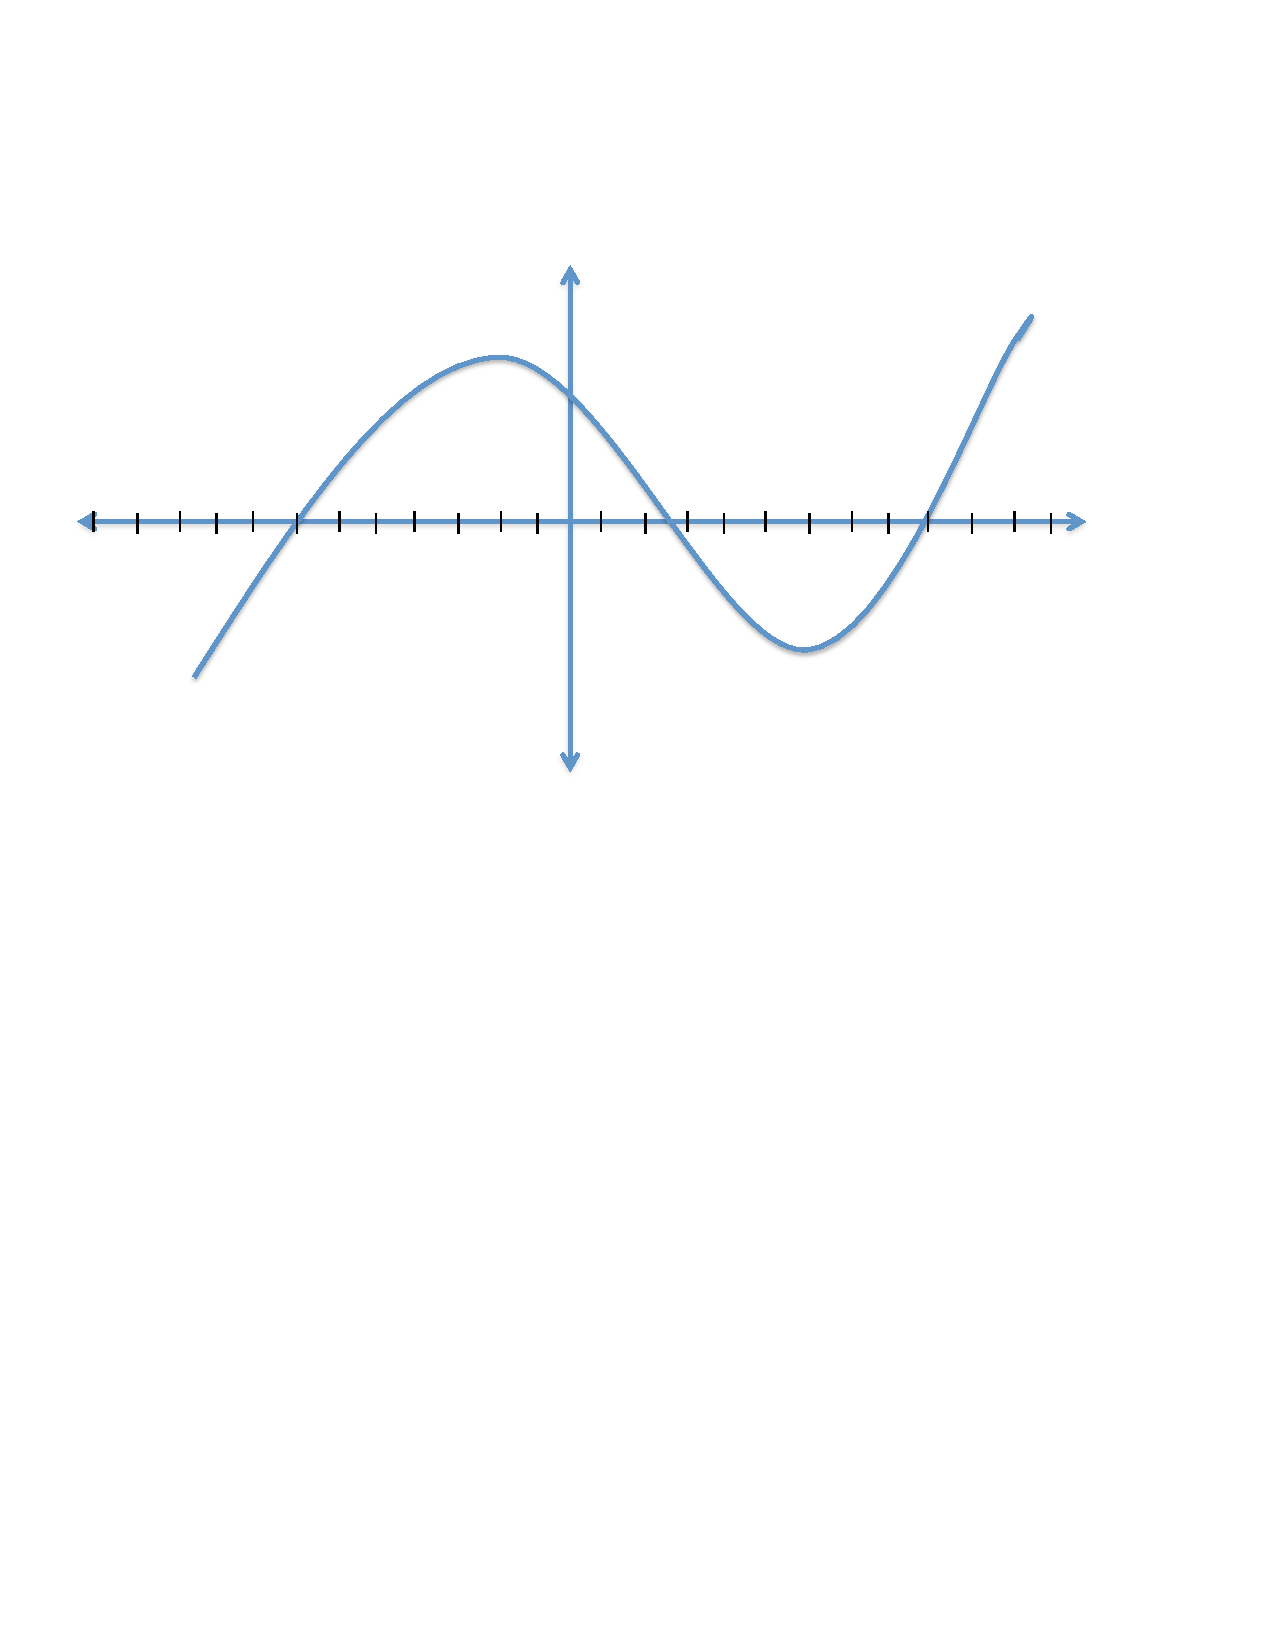
\includegraphics[trim= 140 420 290 180]{Figure2.pdf}
	\end{image}
	
	\begin{enumerate}
	
	%part a
	\item  Describe the motion of the object as precisely as you can.
		\begin{freeResponse}
		Let us assume that $f(t)$ gives the position of John from his house at time $t$.  If $f(t) < 0$, then John is west of his house;  if $f(t) > 0$, then John is east of his house; if $f(t)=0$, then John is in front of his house.  
		
		For the first hour, that is, for $0 \leq t \leq 1$, John walks east away from his house.
		
		\begin{image}
		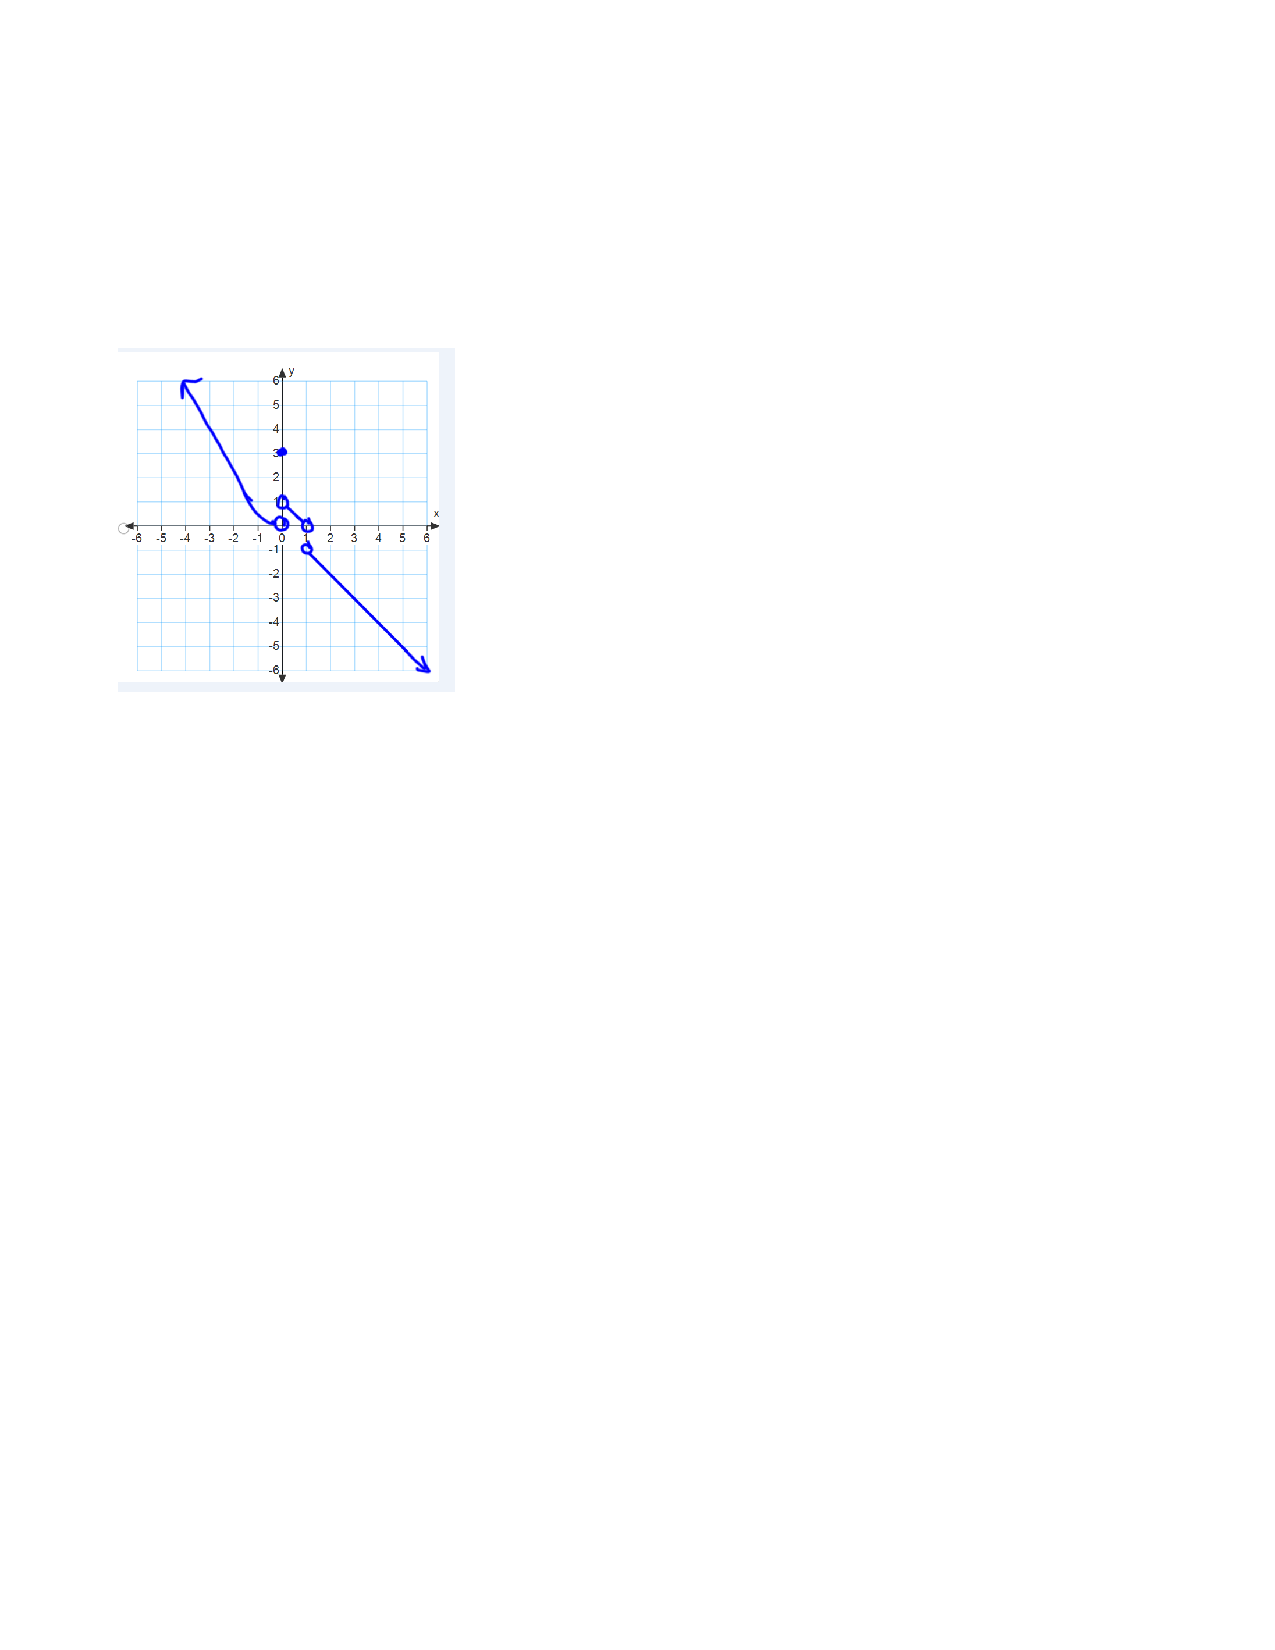
\includegraphics[trim= 140 570 290 200]{Figure3.pdf}
		\end{image}
	
		For the second hour, that is, for $1 \leq t \leq 2$, John turns around and starts walking back west.  However, he does not walk all the way back to his house.
		
		\begin{image}
		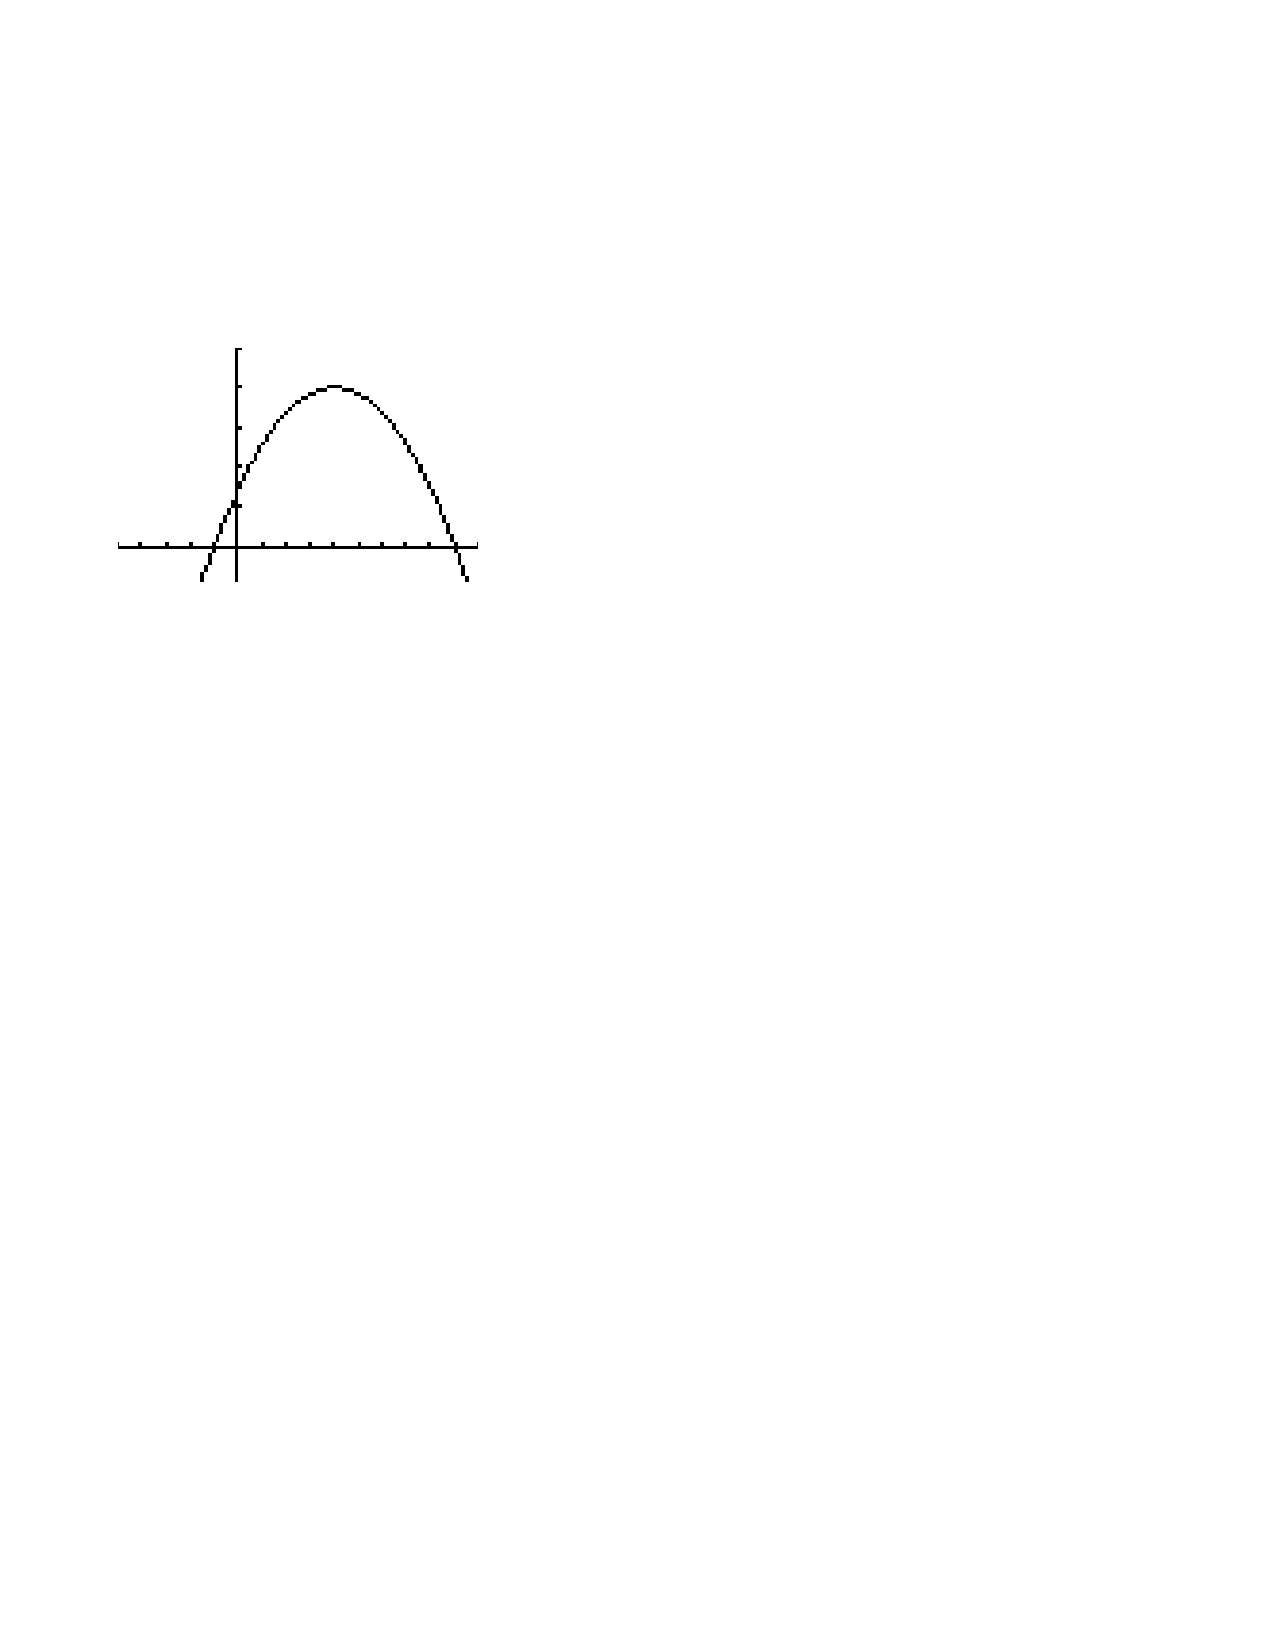
\includegraphics[trim= 140 570 290 200]{Figure4.pdf}
		\end{image}
		
		For the third hour, that is, for $2\le t\le 3$, John realizes he needs to pick up an apple from the grocery store, which is way east of his house, for Elaine.  So he turns around again and walks east to the store.
		
		\begin{image}
		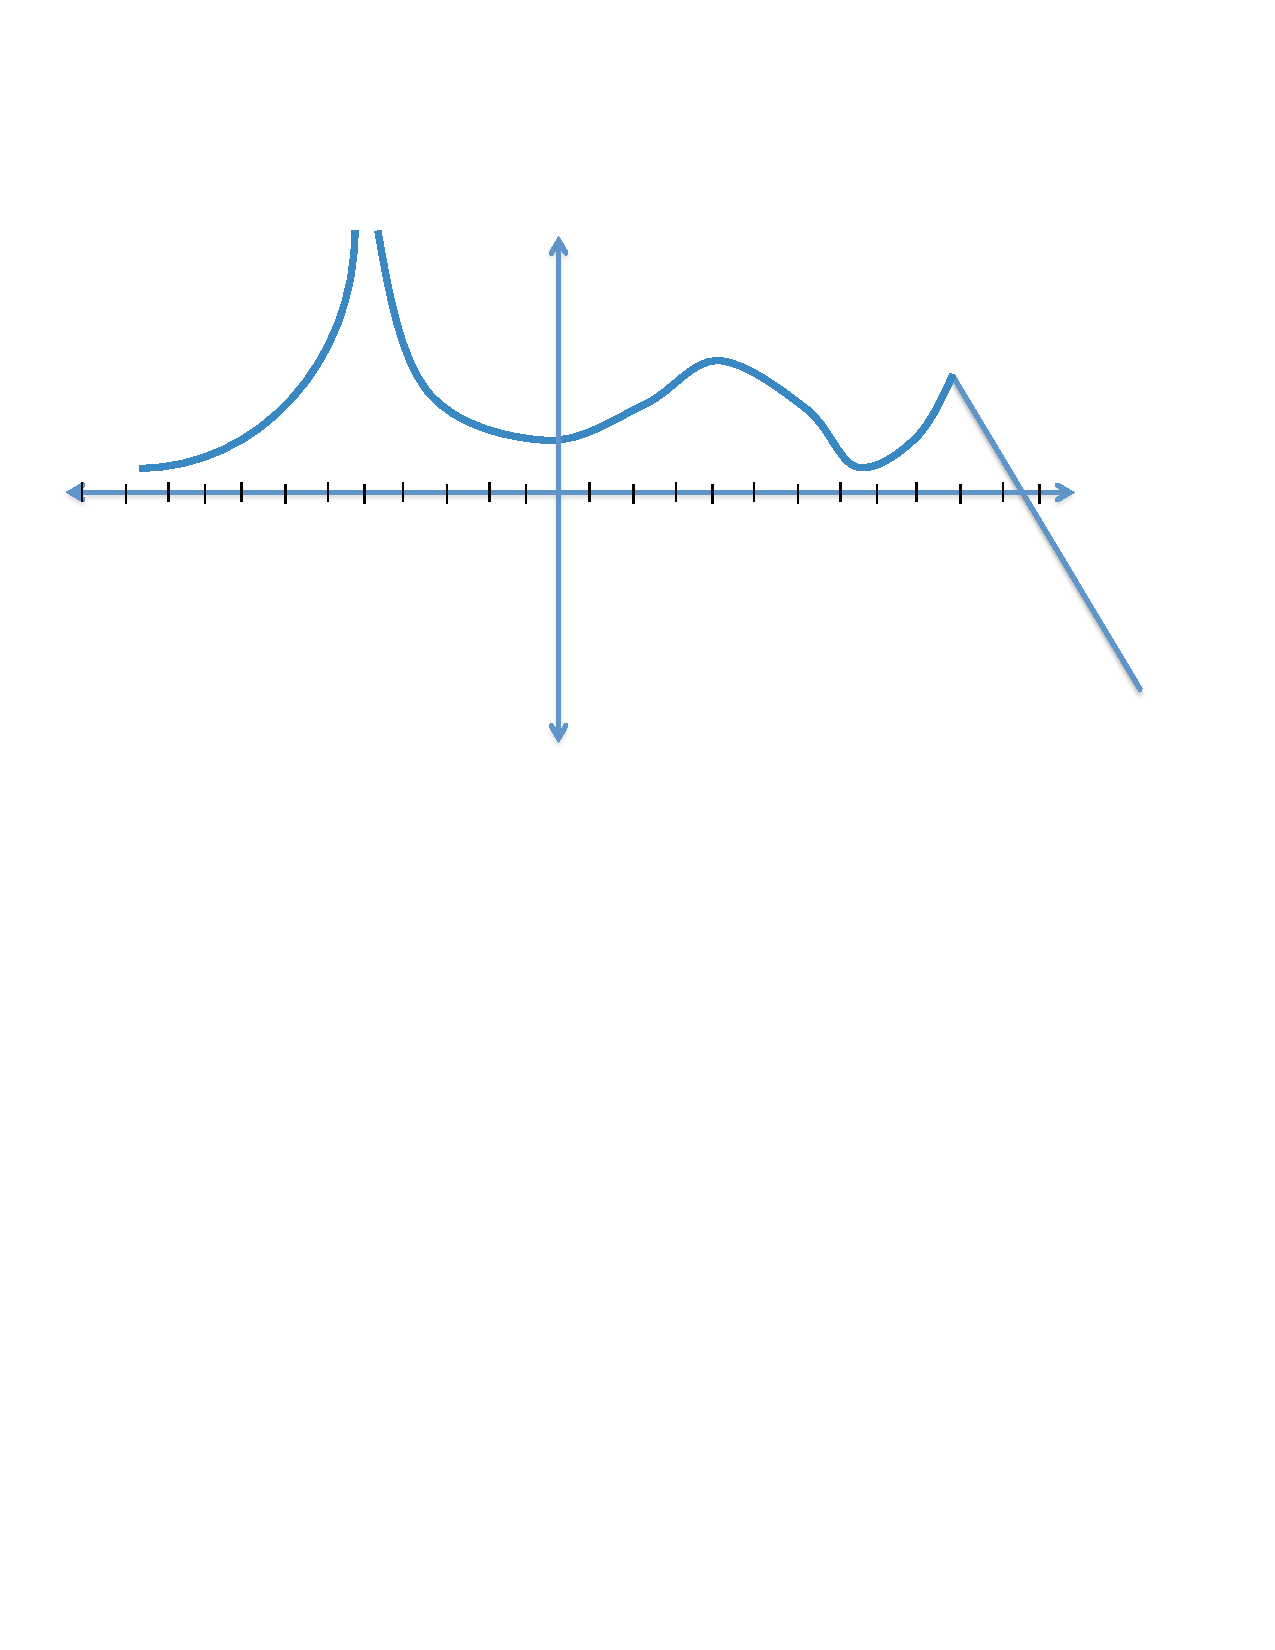
\includegraphics[trim= 140 570 290 200]{Figure5.pdf}
		\end{image}
		
		For the fourth hour, that is, for $t \ge 3$, John needs to drop the apple off at Elaine's house, which is west of his house.  He turns west and walks past his house until he makes it to Elaine's house.
		
		\begin{image}
		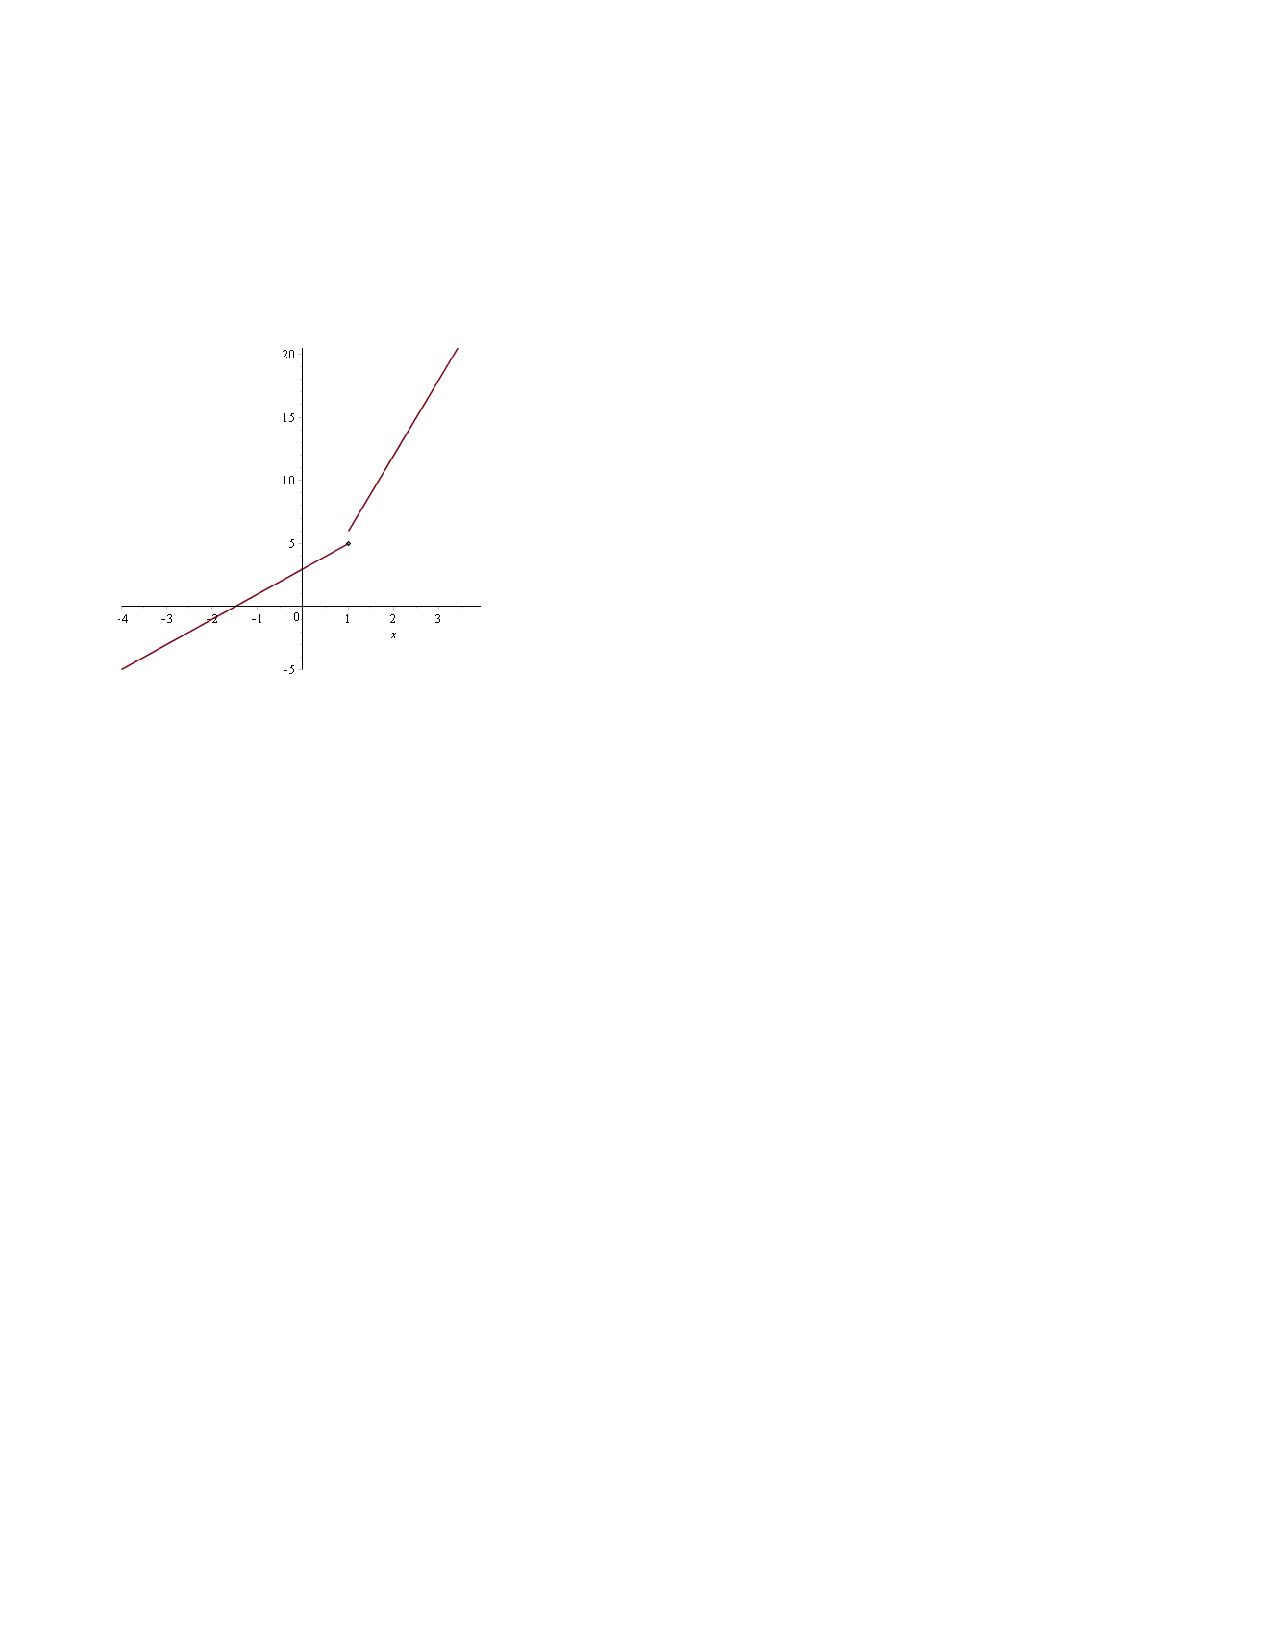
\includegraphics[trim= 140 540 290 200]{Figure6.pdf}
		\end{image}

		\end{freeResponse}
		
		
		
	%part b
	\item  When is the velocity of the object zero?  What is happening to the object at those times? 
		\begin{freeResponse}
		John's velocity is zero at times $t=0,t=1,t=2$, and $t=3$ (the times where the slopes of the tangent lines are zero).  At these times, John changes direction since the slopes of the tangent lines to the graph of $f(t)$ change from positive to negative.
		\end{freeResponse}
		
		
		
	%part c
	\item  When is the object moving in the positive direction?  When is the object the furthest in the positive direction and the furthest in the negative direction?
		\begin{freeResponse}
		John is moving in the positive direction (in this story, east) during times in the region $(0,1) \cup (2,3)$.  John is furthest in the positive direction at time $t=3$ and furthest in the negative direction at (approximately) time $t=3.5$.
		\end{freeResponse}
		
		
		
	%part d
	\item  When is the object speeding up and slowing down? When is the object going at maximum velocity?
		\begin{freeResponse}
		John is speeding up in the region $(0,0.5) \cup (1, 1.5) \cup (2, 2.5) \cup (3, 3.5)$.  He is slowing down in the region $(0.5, 1) \cup (1.5, 2) \cup (2.5, 3)$.  John is moving the fastest at time $t = 3.5$, but that maximizes his speed, not his velocity, because he is moving in the negative direction at that time.  It appears that he maximizes his velocity at about $t=2.5$.  
		\end{freeResponse}
		
		
		
	\end{enumerate}
			
			
	
\end{problem}
















%problem 5
\begin{problem}
Suppose that a stone is thrown vertically upward from a cliff on Mars with an initial velocity of $64$ ft/s from a height of $192$ ft.  The height $s$ of the stone above the ground after $t$ seconds is given by $s(t) = -6t^2 + 24t + 192$.

	\begin{enumerate}
	
	%part a
	\item  Determine the velocity and acceleration of the stone after $t$ seconds.
			\begin{freeResponse}
			The velocity $v(t)$ is:  $v(t) = s'(t) = -12t + 24$.
			
			The acceleration $a(t)$ is:  $a(t) = v'(t) = s''(t) = -12$.
			\end{freeResponse}
			
			
			
	%part b
	\item  What is the greatest height of the stone and when does it occur?  What are the velocity and acceleration at that time?
			\begin{freeResponse}
			Since the function $s(t)$ is differentiable everywhere (it is a polynomial), the maximum height must occur at a time when the velocity is $0$.  So we solve:
			\begin{align*}
			v(t) = -12t+24 &:= 0 \\
			12t &= 24 \\
			t &= 2
			\end{align*}
			
			It is easy to check that $v(t) > 0$ for $0 \leq t < 2$ and $v(t) < 0$ for $2 < t$, and so the greatest height of the stone really does occur at time $t=2$.  The greatest height is $s(2) = -24 + 48 + 192 = 216$ ft.  For the second question we have already seen that $v(2) = 0$ ft/sec, and we have a constant acceleration of $-12$ ft/sec$^2$.  So $a(2) = -12$ ft/sec$^2$.
			\end{freeResponse}
			
			
			
	%part c
	\item  When does the stone hit the ground?  What are the velocity and acceleration at that time?
			\begin{freeResponse}
			The stone hits the ground when $s(t) = 0$.  So we solve:
			\begin{align*}
			s(t) = -6t^2 + 24t + 192 &:= 0 \\
			-6(t^2 - 4t - 32) &= 0 \\
			-6(t-8)(t+4) &= 0 
			\end{align*}
			
			Since we are only considering $t \geq 0$, we must have $t=8$.  At this instant, $v(8) = -96 + 24 = -72$ ft/sec and $a(8) = -12$ ft/sec$^2$.  
			
			\end{freeResponse}
			
			
			
	\end{enumerate}
			
			
			
		
\end{problem}
	


	
	
	
	
	
	
	
	
	

	










								
				
				
	














\end{document} 


















